\chapter{MODELO PROPOSTO}

Foi proposta a execução do projeto em seis partes descritas a seguir. 

\section{\textbf{Simulação dos circuitos}}

O LTspice é um software de simulação que pode ser utilizado para simular e analisar o comportamento e funcionamento de um circuito elétrico, contendo uma grande variedade de componentes  como, por exemplo, transistores, diodos, resistores e capacitores \cite{Spice}.

Esta ferramenta possibilita que o usuário estime com bastante precisão, através de vários tipos de simulações, o comportamento de circuitos elétricos dos mais variados tamanhos e níveis de complexidade.
Para que o SPICE possa realizar tais estimativas, via simulação, o usuário deve fornecer ao software os seguintes dados\cite{LTSpice}:
\renewcommand{\theenumi}{\Alph{enumi}}
 \begin{enumerate}
\item  Descrição do circuito: Elementos, fontes de sinais e de polarização, e principalmente como estes dispositivos estão interligados no circuito. É necessário o fornecimento dos parâmetros modelares para a descrição comportamental dos componentes ativos a serem simulados.

\item  Especificação de análise: Tipos de análise a serem executadas (CC, transiente, pequenos sinais etc.)

\item  Especificação dos resultados: Tipo de resultado esperado da simulação, como correntes e tensões específicas.
\end{enumerate}

Um dos grandes diferenciais do LTspice é a possibilidade de programar o comportamento dos componentes no decorrer da simulação. Assim é possível, através de configurações de parâmetros, induzir comportamentos imprevistos, simular a resposta para condições extremas ou fornecer diferentes tipos de entrada dentre outras alterações. 

Devido às características apresentadas, este  foi o simulador escolhido para o projeto. Foram usadas quatro topologias conhecidas para a obtenção dos dados, dentro das quais foram escolhidos, aleatoriamente, componentes cujos valores sofreram variações durante a simulação (ora com valores altos, ora com valores extremamente baixos). Estas alterações objetivam provocar falhas que influenciam na tensão de saída do sistema, sendo cada falha provocada de forma única e isolada. 


\begin{enumerate}
    \item[Circuito I - ] \textbf{\textit{Sallen Key:}} Este é um circuito passa-banda ativo de 2ª Ordem, projetado neste trabalho com 1 amplificador operacional como o núcleo do circuito, 5 resistores e 2 capacitores, a qual é a configuração mais básica deste tipo de arquitetura. A sua arquitetura é mostrada na \ref{fig:Circuito1}. Este é o principal circuito utilizado no estudo de detecção de falhas, devido à sua baixa sensibilidade aos parâmetros passivos do circuito \cite{Cbrn2009}. 


\begin{figure}[H]
\begin{center}
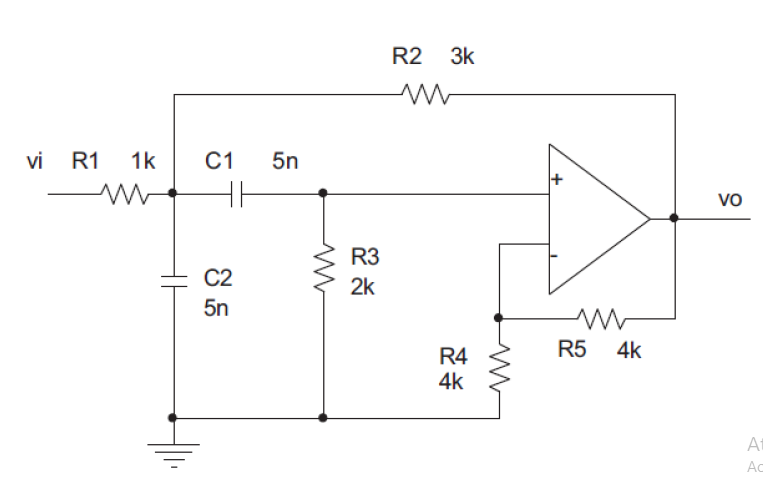
\includegraphics[width=12cm]{./04_Cap4/figures/sallenckt.png}
\caption{\label{fig:Circuito1}- Circuito :{\textit{ Sallen Key}}}
\end{center}
\end{figure}

 
Para simular falhas neste circuito são realizadas alterações nos valores dos resistores R1, R2 e R3  e dos capacitores C1 e C2. Essa variação esta visível na \ref{tab:falhasckt1}.

 \begin{table}[H]
         \centering
        \begin{tabular}{ccc}
        \textbf{Grupo} & \textbf{Simulação} & \textbf{Classificação do Erro} \\
   1              & 0-299              & R1 Alto                        \\
        2              & 300-599            & R1 Baixo                       \\
        3              & 600-899            & R2 Alto                        \\
        4              & 900-1199           & R2 Baixo                       \\
        5              & 1200-1499          & R3 Alto                        \\
        6              & 1500-1799          & R3 Baixo                       \\
        7              & 1800-2099          & C1 Aberto                      \\
        8              & 2100-2399          & C1 Curto                       \\
        9              & 2400-2699          & C2 Aberto                      \\
        10             & 2700-2999          & C2 Curto                       \\
        11             & 3000-3299          & Normal                     \end{tabular}
        \caption{\label{tab:falhasckt1}- Falhas circuito 1}
\end{table}  


    

 \item[Circuito II - ]    \textbf{\textit{Biquad Highpass Filter}}: O Filtro Passa Alta Ativo de segunda ordem é obtido com 4 amplificadores operacionais na parte ativa do circuito, 10 resistores e 2 capacitores, totalizando 12 componentes passivos e 16 componentes no total. A sua arquitetura é mostrada na \ref{fig:Circuito2}. Este circuito também é bastante utilizado no estudo de detecção de falhas por sua baixa sensibilidade à variação dos parâmetros passivos \cite{lombardi} . 
 

    
\begin{figure}[H]
\begin{center}
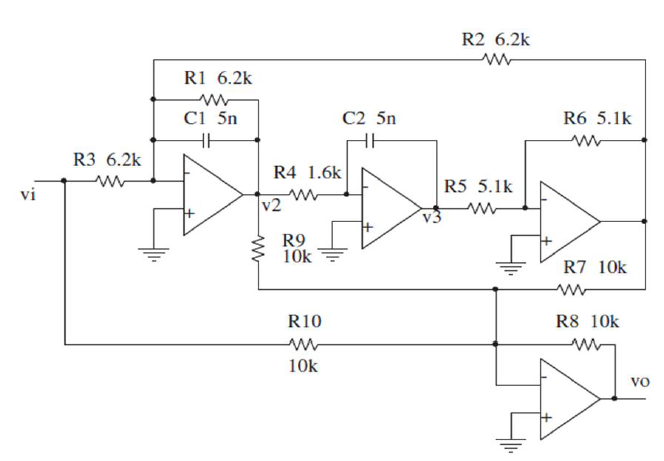
\includegraphics[width=12cm]{./04_Cap4/figures/bickt.png}
\caption{\label{fig:Circuito2}- Circuito: {\textit{Biquad Highpass Filter}}}
\end{center}
\end{figure}

Para simular falhas neste circuito varia-se os valores dos resistores R1, R2, R3 e R4  e dos capacitores C1 e C2.Essa variação esta visível na \ref{tab:falhasckt2}. 

 \begin{table}[H]
         \centering
        \begin{tabular}{ccc}
        \textbf{Grupo} & \textbf{Simulação} & \textbf{Classificação do Erro} \\
        1              & 0-299              & R1 Alto                        \\
        2              & 300-599            & R1 Baixo                       \\
        3              & 600-899            & R2 Alto                        \\
        4              & 900-1199           & R2 Baixo                       \\
        5              & 1200-1499          & R3 Alto                        \\
        6              & 1500-1799          & R3 Baixo                       \\
        7              & 1800-2099          & R4 Alto                      \\
        8              & 2100-2399          & R4 Baixo                       \\
        9              & 2400-2699          & C1 Aberto                      \\
        10             & 2700-2999          & C1 Curto                       \\
        11             & 3000-3299          & C2 Aberto                      \\
        12             & 3300-3599          & C2 Curto                       \\
        13             & 3600-3899         & Normal                        
        \end{tabular}
        \caption{\label{tab:falhasckt2}- Falhas circuito 2}
\end{table}

\item[Circuito III - ] 
\textbf{\textit{CTSV (Continuous-Time State-Variable):}} O filtro universal é um circuito projetado com 3 amplificadores operacionais em sua parte ativa, 7 resistores e 2 capacitores, totalizando 9 componentes passivos e 12 componentes no total. A sua arquitetura é mostrada \ref{fig:Circuito3}. Depois do Sallen-Key, este é um dos principais circuitos utilizados no estudo de detecção de falhas pelos mesmos motivos do Sallen-Key. \cite{lombardi} 

\begin{figure}[H]
\begin{center}
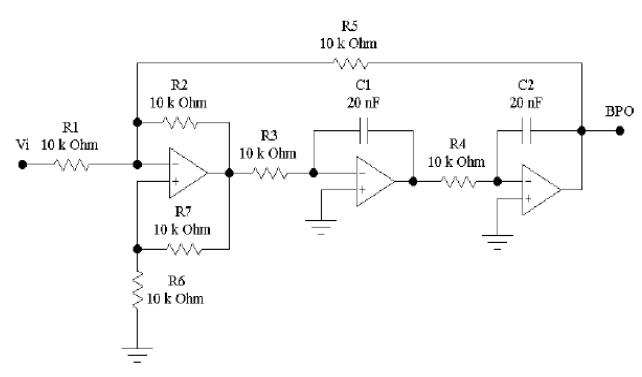
\includegraphics[width=12cm]{./04_Cap4/figures/ctsvckt.png}
\caption{\label{fig:Circuito3}- Circuito: {\textit{ Continuous-Time State-Variable.}}}
\end{center}
\end{figure}

Para simular falhas neste circuito alterna-se os valores dos resistores R1, R2, R3, R4, R5, R6 e R7 e dos capacitores C1 e C2. Essa variação esta visível na \ref{tab:falhasckt3}.
 
 

 \begin{table}[H]
         \centering
        \begin{tabular}{ccc}
        \textbf{Grupo} & \textbf{Simulação} & \textbf{Classificação do Erro} \\
        1              & 0-299              & R1 Alto                        \\
        2              & 300-599            & R2 Baixo                       \\
        3              & 600-899            & R2 Alto                        \\
        4              & 900-1199           & R2 Baixo                       \\
        5              & 1200-1499          & R3 Alto                        \\
        6              & 1500-1799          & R3 Baixo                       \\
        7              & 1800-2099         & R4 Alto                        \\
        8              & 2100-2399          & R4 Baixo                       \\
        9              & 2400-2699          & R5 Alto                        \\
        10             & 2700-2999          & R5 Baixo                       \\
        11             & 3000-3299         & R6 Alto                        \\
        12              & 3300-3599          & R6 Baixo                       \\
        13              & 3600-3899          & R7 Alto                        \\
        14             & 3900-4199          & R7 Baixo                       \\
        15              & 4500-4799         & C1 Aberto                      \\
        16              & 4800-5099         & C1 Curto                       \\
        17              & 5100-5399         & C2 Aberto                      \\
        18               & 5400-5699        & C2 Curto                       \\
        19              & 5700-5999         & Normal                        
        \end{tabular}
        \caption{\label{tab:falhasckt3}- Falhas circuito 3}
\end{table}


\item[Circuito IV - ]\textbf{\textit{ Nonlinear Rectfier:}} Dos 4 circuitos descritos, o retificador não-linear é o único que não é um circuito de filtro e por consequência o circuito mais sensível às variações dos seus parâmetros. A sua arquitetura pode ser vista na \ref{fig:Circuito4}. Não possui componentes ativos e é composta por um único diodo retificador, três capacitores, um indutor e uma resistência \cite{Clayton}.

\begin{figure}[H]
\begin{center}
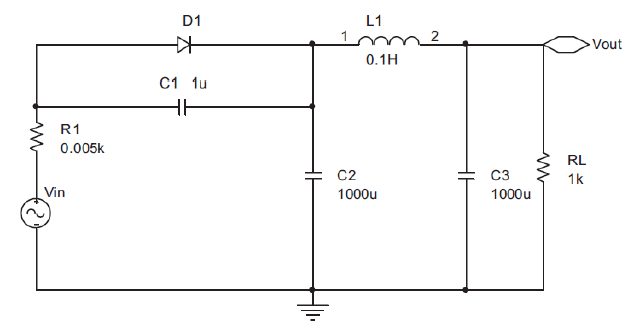
\includegraphics[width=12cm]{./04_Cap4/figures/retificadorckt.png}
\caption{\label{fig:Circuito4}- Circuito:{\textit{ Nonlinear Rectfier}.}}
\end{center}
\end{figure}
Para simular falhas neste circuito provoca-se a variação dos valores dos resistores R1, capacitores C1, C2 e C3 e indutor L1.Essa variação esta visível na \ref{tab:falhasckt4}.

 \begin{table}[H]
         \centering
        \begin{tabular}{ccc}
        \textbf{Grupo} & \textbf{Simulação} & \textbf{Classificação do Erro} \\
        1              & 0-299              & R1 Alto                        \\
        2              & 300-599            & R1 Baixo                       \\
        3              & 600-899            & C1 Aberto                        \\
        4              & 900-1199           & C1 Curto                       \\
        5              & 1200-1499          & C2 Aberto                        \\
        6              & 1500-1799          & C2 Curto                       \\
        7              & 1800-2099          & C3 Aberto                      \\
        8              & 2100-2399          & C3 Curto                       \\
        9              & 2400-2699          & L1 Aberto                      \\
        10             & 2700-2999          & L1 Curto                       \\
        11             & 3000-3299          & Normal                        
        \end{tabular}
        \caption{\label{tab:falhasckt4}- Falhas circuito 4}
\end{table}



\end{enumerate}

Ao simular-se os circuitos segundo parâmetros pré-configurados (tempo de processamento, quantidade de simulações para cada estágio, valores dos componentes, entre outros) a saída dos dados, para todos os nós, é exportada para um arquivo \textit{".raw"}.

\section{\textbf{Leitura dos dados de entrada}}

Para realizar a leitura do arquivo de extensão \textit{".raw"}, exportado pelo LTSpice, é necessário conhecer uma série de instruções sobre os métodos de composição do arquivo. Este arquivo é uma combinação de diferentes estruturas e informações do circuito, armazenadas e comprimidos de modos diferentes.

O desenvolvimento de um processo específico para a leitura deste tipo de arquivo se faz necessário pela falta de uma biblioteca na linguagem que seja destinada especificamente para a leitura de arquivos nativos do LTSpice. 

A primeira linha de qualquer arquivo \textit{".raw"} começará com características da simulação e caminho do sistema, onde se encontra o arquivo de simulação. Por exemplo: 

"
Title: * C:\textbackslash \textbackslash Users\textbackslash \textbackslash jessi\textbackslash \textbackslash PycharmProjects\textbackslash \textbackslash ProjetoFinal\textbackslash \textbackslash Sallen Key mc + 4bitPRBS [FALHA].asc

Date: Wed Jul 25 23:33:14 2018

Plotname: Transient Analysis

Flags: real forward stepped

No. Variables: 42

No. Points:      2943376

Offset:   0.0000000000000000e+000

Command: Linear Technology Corporation LTspice IV

Backannotation: u1 1 2 3 4 5
"


Em seguida o arquivo escreve uma lista com todas as variáveis registradas e armazenadas no circuito. 

Exemplo:

Variables:

	0 & time &	time
	
	1 &	V(clock) &	voltage
	
	2 & 	V(n002) &	voltage
	
	3	V(n004)	voltage
	
	.
	.
	.
	
	40	Ix(u1:4)	subckt_current
	
	41	Ix(u1:5)	subckt_current



A terceira parte do arquivo \textit{".raw"}, finalmente, contém os dados. Eles são armazenados em representação binária e com tamanho proporcional aos dados gerados pela simulação e pelas configurações do programa. Ou seja, existe um alto grau de complexidade para se extrair os dados da simulação e montar um \textit{objeto} (estrutura de dados que lista valores pertinentes a categorizações) devido a incerteza e grande variedade de formato dos dados a serem obtidos. 

Para concluir o processo de aquisição de dados foi usado como base um código ainda incompleto, mas já disponibilizado no \textit{Github} por um desenvolvedor \cite{nuno}, acrescido de várias manipulações de dados. 

Um fator importante a ser destacado é a grande quantidade de dados trabalhada. São processados em torno de 800 milhões de valores ao todo nos quatro circuitos. 


\begin{figure}[H]
\begin{center}
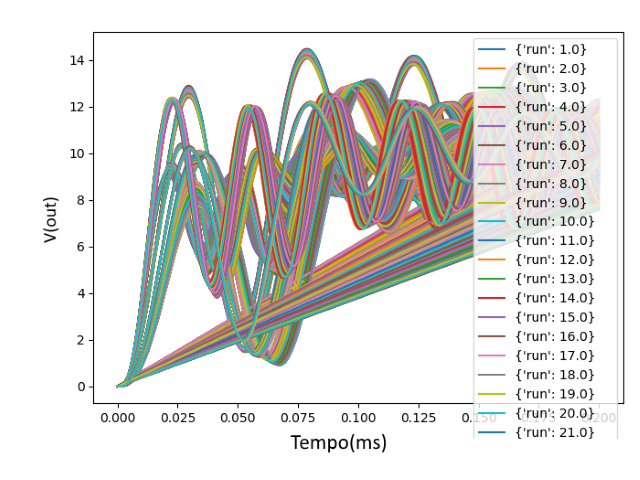
\includegraphics[width=15cm]{./04_Cap4/figures/DadosBrutosNONLinear.png}
\caption{\label{fig:SallenBruto}-Dados Brutos da tensão de saída (Vout x Time)}
\end{center}
\end{figure}


Com os dados inseridos e organizados, foi necessária uma nova etapa: a limpeza e armazenamento dos dados em um CSV. 

Como esse processo de leitura, levando em conta todas as variáveis apresentadas na seção anterior são computacionalmente trabalhosos e demorados, escolheu-se fazer a escrita desses dados em um aquivo CSV para agilizar os testes e compilações posteriores.

Entretanto, para esses dados poderem ser escritos corretamente nas linhas e colunas, preservando os dados desejados e excluindo os valores de variáveis desnecessárias para nosso processo, foi utilizado a técnica de ETL (Extração, transformação e limpeza) \cite{selecao}.

Os dados inicialmente apresentavam, para alguns casos, inconsistências como valores inesperados, formato inadequado, incoerência no relacionamento com a variável tempo, quantidade  diferente de dados para simulações semelhantes entre outros. 

Toda essa manipulação de dados foi desenvolvida utilizando bibliotecas como Pandas e  Numpy, além de bastante manipulação dos dataFrames criados. 

Após esses ajustes e salvando no CSV apenas as variáveis de interesse, conseguimos reduzir os dados para 18 milhões. Só essa alteração já gerou uma grande mudança na velocidade de processamento:  2,25\% dos dados iniciais passam para as próximas fases.
 

\section{\textbf{Extração de Assinaturas (PAA)}}

O passo seguinte foi a aplicação do método de reduzir o numero de dados significativos da simulação. Para isso é usado o PAA (Piecewise Aggregate Approximation – PAA). 

O Aproximação Agregada por Partes (Keogh et al., 2000) é uma técnica de redução de dimensão que é bastante simples de entender e implementar. Ela permite diferentes medidas de distância e apresenta resultados competitivos quando comparada a transformações mais sofisticadas como a decomposição por valor singular (SVD – Singular Value Decomposition) e as Transformadas de Fourier e Wavelet, na tarefa de indexação das séries temporais (Keoghet al., 2000). Uma série temporal (senoidal)
\begin{equation}
X=x_{1},...,x_{n} \end{equation} pode ser representada no espaço N, n \leqslantn ,
\begin{equation}
\overline{X}=\overline{x_{1}},...,\overline{x_{n}}
\end{equation}
\begin{equation}
\overline{x_{i}}= \frac{N}{n}\sum_{j=\frac{N}{n}(i-1)+1}^{\frac{N}{n}i}x_{j}
\end{equation}
A Equação indica que o sinal é dividido em N janelas (segmentos) e que o valor médio representa todos os pontos nesta janela. A \ref{fig:PAASaplicacao} mostra o sinal de uma simulação e sua respectiva representação PAA. O numero de segmentos desejado é uma variável do algoritmo. \cite{timeSerial}. 

\begin{figure}[H]
\begin{center}
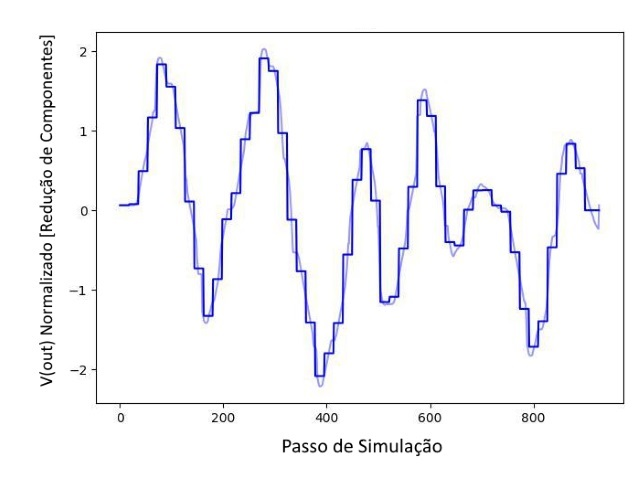
\includegraphics[width=14cm]{./04_Cap4/figures/paa-simples.jpg}
\caption{\label{fig:PAASaplicacao}- Aplicação do PAA (Vout x Time)}
\end{center}
\end{figure}

O método é aplicado a todo DataFrame, diminuindo significamente o número de pontos necessários para representar a simulação e ainda preservar com qualidade o comportamento do modelo. Na \ref{fig:Analisepaa} temos o conjunto de todos os dados de entrada do circuito antes de depois do PAA. Neles há uma redução de 90\% no na variação dos dados, mas mesmo assim eles continuam com o mesmo perfil e agregando bastante dificuldade de os diferenciar, mostrando como o PAA é eficiente ao que se propõe. 

\begin{figure}[H]
\begin{center}
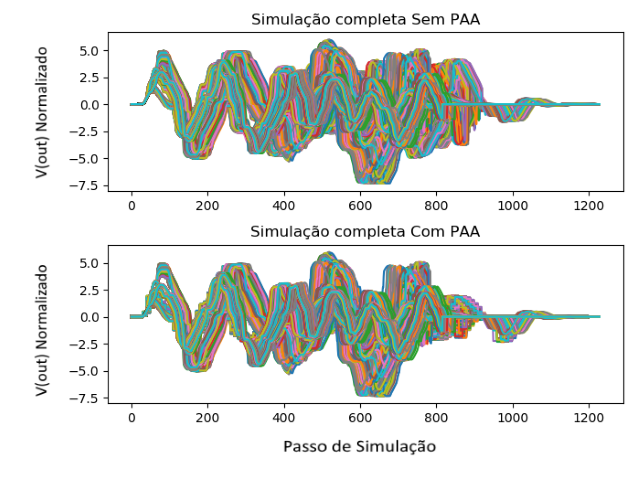
\includegraphics[width=15cm]{./04_Cap4/figures/dadosCompletos.png}
\caption{\label{fig:Analisepaa}- Comparação do Vout antes de depois do PAA (Vout x Time).}
\end{center}
\end{figure}


\section{\textbf{Análise das Componentes Principais (PCA)}}

A Análise das Componentes Principais é a observação do conjunto de dados em um novo espaço, onde este novo conjunto de dados não é linearmente correlacionado. O espaço é definido a partir dos autovalores e autovetores da matriz de covariância dos dados.
Fazendo a covariância das funções no espaço mapeado em x, obtém-se:

\begin{equation}

    {\overline{C}=\frac{1}{n}\sum_{��=1}^{1}\varphi (xi).\varphi (xi)^{T}}
\end{equation}

Temos então que é a matriz de covariância é dada por:

\begin{equation}

\overline{C}=\left[
\begin{array}{c c c}
c_{11}&\ldots& a_{1n}\\
\vdots&\ddots &\vdots\\ c_{n1}&\ldots& c_{nn}
\end{array}\right]

\end{equation}
e
\begin{equation}
c_{ij}=\varphi (xi).\varphi (xi)^{T}

\end{equation}

A aplicação do PCA aconteceu com o auxilio do modulo de PCA da biblioteca sklearn. 


Seguindo seus passos previstos, o PCA base foi calculado através no numero de colunas do dataframe. Esse será por definição o limite de componentes de variância que o método pode ter \cite{pca}. 

Aplica-se um teste para descobrir o numero de componentes necessários para termos uma boa taxa de variância dos dados. 

exemplo do circuito Sallen Key : 

Variância total dos primeiros 1 componentes: 0.38993472912639116

Variância total dos primeiros 2 componentes: 0.6049460165428534

Variância total dos primeiros 3 componentes: 0.7264523762053858

Variância total dos primeiros 4 componentes: 0.8200175327019206

Variância total dos primeiros 5 componentes: 0.8697641955453185

Variância total dos primeiros 6 componentes: 0.8979201818957931

Em seguida insere-se o valor final do número de componentes a serem usados e obtém como resposta os dados reduzidos. 

\begin{figure}[H]
\begin{center}
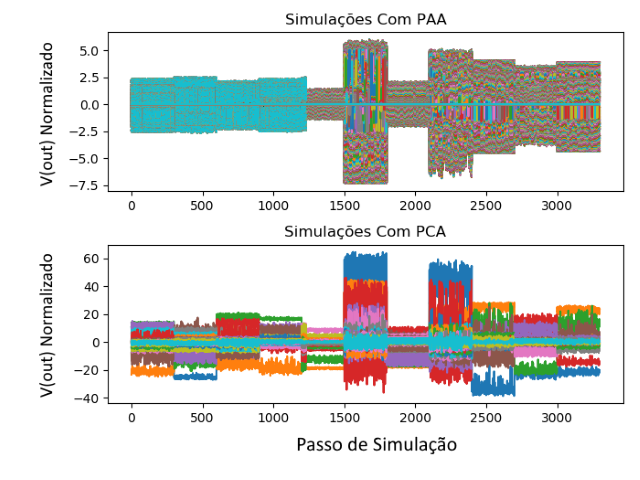
\includegraphics[width=15cm]{./04_Cap4/figures/reducaoPCA.png}
\caption{\label{fig:PCAreducao}- Simulação antes e após o PCA (Vout x Time).}
\end{center}
\end{figure}

Nessa analise é visível como os dados preservam as características, mesmo tendo uma  redução extremamente significativa. O objetivo desse processo de redução é exatamente esse, pegar as principais e mais significativas componentes para as preservar. Essa análise é realizada ao visualizarmos que cada cor significa uma  simulação, a imagem inicial apresenta uma elevada densidade de cores, no segundo caso, essa densidade é diminuída chegando a ter áreas em branco oficializando a redução da quantidade de dados. 

Observando os dados limpos, já é possível perceber diferenças de comportamento para diferentes momentos, já nos aproximando da detecção das falhas. 


\section{\textbf{Aplicação da aprendizagem de maquinas}}

A detecção é realmente realizada nesta etapa do processo. O subsistema consiste basicamente de um classificador e do conjunto de dados processados de características. Antes da real execução da detecção, os dados de resposta do circuito são utilizados para o treinamento do classificador, obtendo o ajuste da sua fronteira de decisão. A seguir, é realizada a detecção para um circuito qualquer, de topologia equivalente aos circuitos treinados. Nesse caso, a saída do classificador corresponderá à saída do sistema de detecção, acusando um determinado defeito ou não no circuito conforme a pertinência do dado obtido à fronteira de decisão do classificador.



Caso desejam-se apenas definir se o circuito apresenta falha ou não, o classificador irá necessitar somente de uma única classe (LI, X., XIE, Y., 2013), não havendo a identificação da falha neste caso. No sistema proposto, é desejado que a detecção não só determine a existência ou não de falha nos circuitos, como também seja capaz de identificá-las. Neste caso, mais classes serão necessárias, havendo N classes de saída para N falhas do circuito.


\begin{figure}[H]
\begin{center}
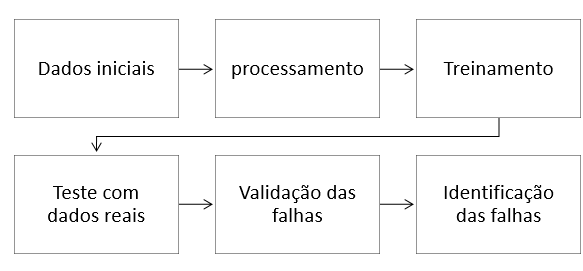
\includegraphics[width=10cm]{./04_Cap4/figures/fluxomachine.PNG}
\caption{\label{fig:fluxomachine}- Diagrama Aprendizado de maquinas}
\end{center}
\end{figure}

A \ref{fig:fluxomachine} exibe o fluxo do dado no processo de aprendizagem. O algoritmo é treinado e depois testado para analisarmos sua taxa de acerto. Após essa etapa, as falhas são identificadas e categorizadas. 

Foram usados 8 algoritmos apresentados no Capitulo 3. Assim podemos diagnosticar quais tem a melhor eficiência para nosso conjunto de dados levando em conta os resultado para os diferentes circuitos. 


\section{\textbf{Validação dos resultados}}

Para avaliar o desempenho dos classificadores primeiro é preciso determinar a porcentagem de falsos positivos e de falsos negativos,ao invés de se analisar apenas a taxa de acerto. Sendo assim, a fração de falsos negativos é definida a priori (fração de rejeição) para a construção do modelo (classificador).
Uma vez que o modelo foi determinado, ele pode ser avaliado em um conjunto de teste e calcular a porcentagem de falsos positivos e falsos negativos. Ainda conforme (Tax, 2008) na literatura existem duas outras medidas que são geralmente usadas: o precision, que é definido na Equação, e o recall, que é basicamente a taxa de verdadeiros positivos e é mostrado na Equação 

\[precision= \text {números de previsões corretas}\div{\text {número de previsões}}\]

\[recall= \text {números de previsões corretas}\div{\text {número de exemplos}}\]


A partir das definições de precision e recall pode-se definir F1 que é uma métrica de
desempenho que está definida na Equação . O F1 relaciona as métricas precision e recall
e essas duas métricas possuem valores no intervalo entre zero e um. Considerando apenas a
relação da multiplicação pela soma do precsion e recall e se os valores forem o máximo, isto
é, precision = 1 e recall =1, o valor máximo dessa relação será 0,5 e com o intuito de
normalizar a métrica F1 = 1, a relação entre o numerador e o denominador é multiplicada por
dois. 

O F1 score foi implementado no algoritmo para nos auxiliar na validação dos resultados\cite{lombardi}. 



